\clearpage
%
\counterwithin{figure}{section}
\counterwithin{table}{section}
%
\counterwithin{equation}{section}
%
%
%
\appendix

\pagenumbering{Roman}  %
\pagestyle{plain}

\twocolumn[
  \begin{@twocolumnfalse}
\newpage
\null
\vskip .375in
\begin{center}
  {\Large \bf \inserttitle \\ \vspace{0.5cm} \large Supplementary Material \par}
  %
  \vspace*{24pt}
  {
%
%
%
%
%
%
%
  \par
  }
  %
%
  %
%
\end{center}
\end{@twocolumnfalse}
]



We report a few additional experiments and results that did not fit in the main paper. 
Section~\ref{sec:suppl-data-augmented-toy} shows the effect of data-augmented batches when training a simple toy model.
Sections~\ref{sec:training-hyperparam} and \ref{sec:full-data-augment} list the values of a few hyper-parameters used in our method. 
Section~\ref{sec:ablationretrieval} gives a some more ablation results in the retrieval setting.
Finally, Section~\ref{sec:extra-classif} shows how to use the ingredients of MultiGrain to improve the accuracy of an off-the-shelf pre-trained ConvNet at almost no additional training cost. 
It obtains what appear to be \textbf{the best reported classification results on imagenet-2012} for a convnet with publicly available weights. 

%
%
%
%
%
%
%

\section{Data-augmented batches: toy model \label{sec:suppl-data-augmented-toy}}
We have observed in \Cref{sec:data-augmented-batches,sec:tradeoff-parameter} that training our  architecture (ResNet-50 trunk) with data-augmented batches yields improvements with respect to the vanilla uniform sampling scheme, despite the decrease in  image diversity. 

This observation holds even in the absence of ranking triplet loss, all things being equal otherwise: same number of iterations per epoch, number of epochs, learning rate schedule, and batch size. 
As an example, \cref{fig:suppl-compare-sampling} shows the evolution of the validation accuracy of our network trained under cross-entropy with our training schedule and a $p = 1$ pooling, batches of size 512, with the data augmentation introduced in \cref{sec:experimental-settings}, with uniform batches vs. with batch sampling. 
While initial epochs suffer from the reduced diversity of the batches compared to the uniformly-sampled variant, the reinforced effect on data augmentation compensates for this in the long run, and makes the batch-augmented variant reach a higher final accuracy. 
\begin{figure}
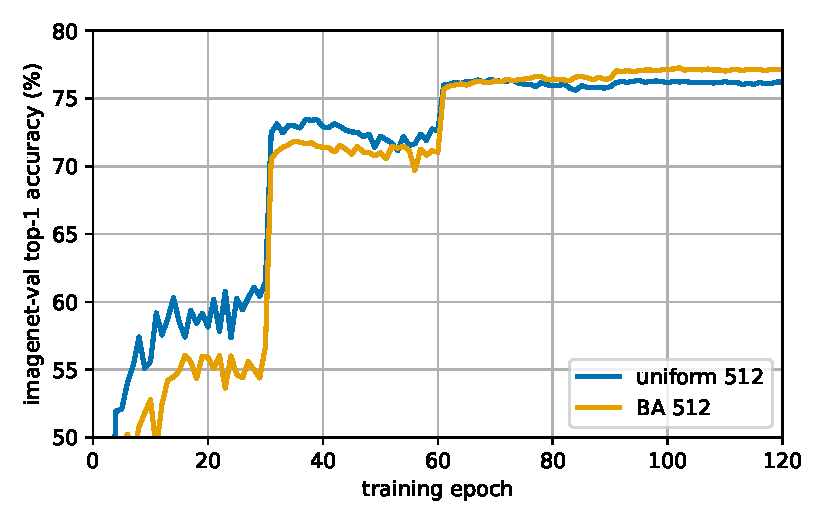
\includegraphics[width=\linewidth]{figs/conv_BA_plot/conv_BA_plot}
\caption{\label{fig:suppl-compare-sampling}
	Evolution of the validation accuracy on ImageNet-val with and without data-augmented batches. 
}
\end{figure}

Since we observe this better performance even for a pure image classification task, an interesting question is whether this benefit is specific to our architecture and training method (batch-norm, etc), or if it is more generally applicable? 
Hereafter we analyse a linear model and synthetic classification task that seems to align with the second hypothesis. 

%

We consider an idealized model of the effect of including different data-augmented instances of the same image in one batch using standard stochastic gradient descent. 
We create a synthetic training set $\mathcal{D}$ of points pictured in \cref{fig:toy-train} of $N$\,=\,$100$ positive and $N$\,=\,$100$ negative training points $\vec{p^i} = (p^i_x, p^i_y)$ by sampling from two 2D Gaussian distributions: 
\begin{equation}
\begin{aligned}
    p_x^i \sim \mathcal{N}(\mu=0, \sigma=1) \\
    p_y^i \sim \mathcal{N}(\mu=y_i^*, \sigma=1)
\end{aligned}
\end{equation}
with $y_i^* = \pm 1$ being the ground truth label. 
We sample a test dataset in the same manner. 

\begin{figure}
\centering
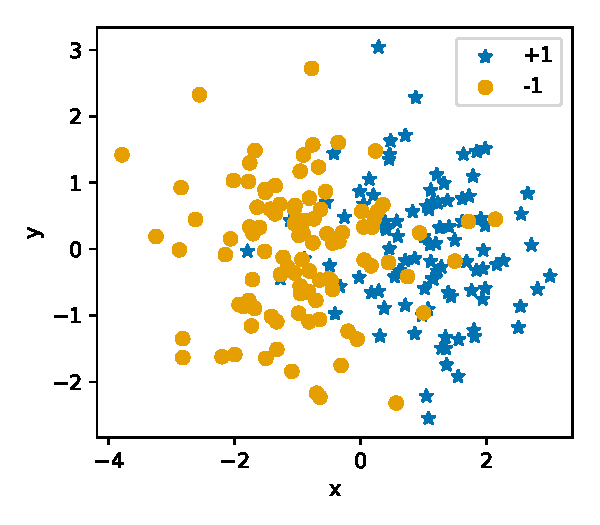
\includegraphics[height=1.5in]{figs/toy/toy_data}
\caption{\label{fig:toy-train}
	Training set for the toy model in~\cref{sec:suppl-data-augmented-toy}.
}
\end{figure}

We consider the SGD training of an SVM
\begin{equation}\label{eq:svm-model}
    f_{\vec{w}}(\vec{p_i}) = \vec{w}^{\top} \vec{p_i}
\end{equation}
using the Hinge loss
\begin{equation}
    \ell^{\text{hinge}} = \max{(1 - y_i^* f_{\vec{w}}(\vec{p_i}), 0)}.
\end{equation}

We consider the symmetry across the x-axis
\begin{equation}
    \phi((p^i_x, p^i_y)) = \phi((p^i_x, -p^i_y))
\end{equation}
as a label-preserving data-augmentation suited to our synthetic dataset. 
We train the SVM~\eqref{eq:svm-model} using one pass through the data-augmented dataset $\bar{\mathcal{D}}$ of size $4N$, using batches of size $2$.

\begin{figure}
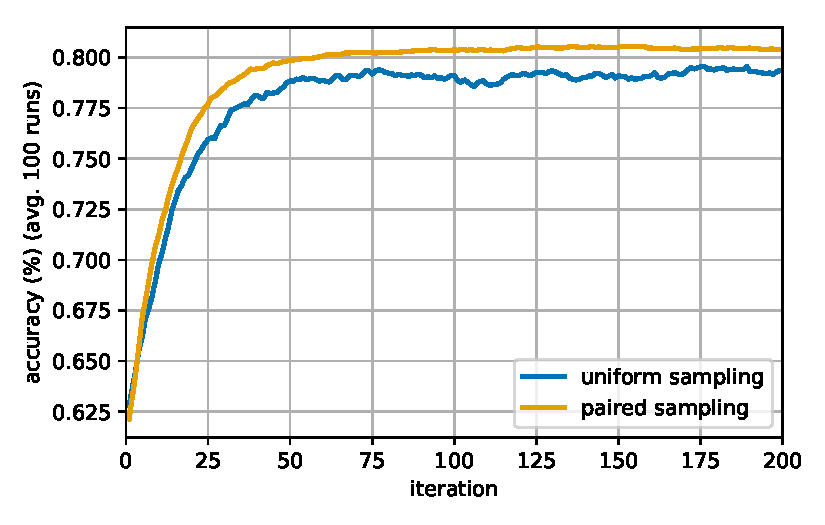
\includegraphics[width=\linewidth]{figs/toy/conv_toy_plot}
\caption{\label{fig:evo-toy}
	Evolution of the test accuracy of the SVM trained on the synthetic data, averaged accross 100 runs.
}
\end{figure}

The only difference between the two optimization schedules is the order in which the samples are batched and presented to the optimizer. 
We consider two batch sampling strategies:
\begin{itemize}
    \item Uniform sampling: we sample the elements of the batch randomly from  $\bar{\mathcal{D}}$, without replacement;
    \item Paired sampling: we generate a batch by pairing a random element from $\bar{\mathcal{D}}$ and its data-augmentation, removing these two elements from $\bar{\mathcal{D}}$.
\end{itemize}
\Cref{fig:evo-toy} shows the evaluation of the accuracy with the iterations in both of these cases, averaged across 100 runs. 
It is clear that pairing the data-augmented pairs in one batch accelerates the convergence of this model. 

This idealized experiment demonstrates that there are cases in which the repeated augmentation scheme provides an optimization and generalization boost, and reinforces the effect of data augmentation.

\section{Margin loss hyper-parameters}

%

%
\label{sec:training-hyperparam}

\Cref{tab:training-hyperparam} 
%
gives the value of the hyper-parameters for the margin loss used during the training of our models.


\begin{table}
\centering
\caption{\label{tab:training-hyperparam}
	Margin loss hyper-parameters
}
%
\begin{tabular}{@{}lc@{}}
\toprule
parameter             & value \\ \midrule
margin $\alpha$       & $0.2$ \\
initial $\beta_0$     & $1.2$ \\
$\beta$ learning rate & $0.1$ \\
\bottomrule
\end{tabular}
%
\end{table}

%
%


\section{Data augmentation hyper-parameters}

%
\label{sec:full-data-augment}

\begin{table}
\centering
\caption{\label{tab:full-data-augment}
	\emph{full} data-augmentation transforms and parameters
}
{\small
\begin{tabular}{@{}lc@{}}
\toprule
\textbf{transformation} & \textbf{parameter range} \\ \midrule
horizontal flip           & \\
\midrule
random resized crop       & \makecell{$\text{scale}\in [0.08, 1.0]$ \\ $\text{ratio}\in [3/4, 4/3]$} \\
\midrule
color jitter & \makecell{brightness $0.3$\\contrast $0.3$\\
saturation $0.3$}\\
\midrule
lighting transform & intensity $0.1$ \\
\bottomrule
\end{tabular}
}
\end{table}

\Cref{tab:full-data-augment} gives the transformations in the \emph{full} data augmentation used in our experiments (\cref{sec:experimental-settings}), along with their parameters. 
%
%
%

\begin{table*}[t]
%
\renewcommand\thetable{D.1}
\centering
\caption{\label{tab:instanceres-abl}
	Full results including Copydays + 10k distractors (CD10k, $\%$~mAP), and ablation study for the MultiGrain models. 
	%
	The Pytorch model simply extract the last activation layer as a descriptor~\cite{babenko2014neural}. 
	Resnet-50 corresponds to features extracted from a 
    classification baseline with $p = 1$ or $p = 3$ GeM pooling, trained with cross-entropy with our training schedule, data augmentation, and uniform batch sampling.
}
%
\def \mysp {\hspace{5pt}}
{\small
%
\begin{tabular}{lc c c@{\mysp}c@{\mysp}c c c@{\mysp}c@{\mysp}c c c@{\mysp}c@{\mysp}c}
\toprule
& & & \multicolumn{3}{c}{Holidays} & &  \multicolumn{3}{c}{UKB} & & \multicolumn{3}{c}{CD10k} \\
\cmidrule(rl){4-6} \cmidrule(rl){8-10} \cmidrule(rl){12-14}
Method & $\lambda$ & $s^*=$ & 224 & 500 & 800 &  & 224 & 500 & 800 &  & 224 & 500 & 800 \\
\midrule
\multicolumn{2}{l}{PyTorch model zoo} & & $85.5$ & $86.6$ & $82.8$ &      & $3.71$ & $3.85$ & $3.80$ &    & $61.5$ & $61.1$ & $43.0$\\
\multicolumn{2}{l}{Resnet-50 trained with $p = 1$ pooling} & & $83.5$ & $88.8$ & $87.1$ &    & $3.60$ & $3.79$ & $3.82$ &    & $59.2$ & $69.9$ & $66.2$\\
\multicolumn{2}{l}{Resnet-50 trained with $p = 3$ pooling} & & $86.8$ & $90.0$ & $90.4$ &    & $3.73$ & $3.87$ & $3.89$ &    & $70.6$ & $78.9$ & $75.7$ \\
MultiGrain & $1$ & & $\bm{88.9}$ & $\bm{91.8}$ & $91.6$ &  & $\bm{3.78}$ & $3.89$ & $\bm{3.91}$ & & $\bm{75.1}$ & $\bm{81.2}$ & $\bm{82.5}$ \\
MultiGrain & $0.5$ & & $88.3$ & $91.5$ & $\bm{92.5}$ & & $\bm{3.78}$ & $\bm{3.90}$ & $\bm{3.91}$ & & $74.1$ & $80.7$ & $78.6$  \\
MultiGrain + AA & $0.5$ & & $86.5$ & $90.3$ & $89.4$ & & $3.75$ & $3.89$ & $3.90$ & & $69.7$ & $77.8$ & $76.1$  \\
\bottomrule
\end{tabular}

%
%
%
%
%
%
%
%
%
%
%
%
%
%
%
%
%
%
%
%
%
%
%
%
%




%
%
%
%
%
%
%
%
%
%
%
%
%
%
%
%
%
%
%
%
%



%
%
%
%
%
%
%
%
%
%
%
%
%
%
%
%
%
%
%
%
%
%
%
%
%
%
%
%
%
%
%
%
%
%
%
%
%
%
%
%

%
%
%
%
%
%
%
%
%
%
%
%
%
%
%
%
%
%

}
\end{table*}


\section{Additional results and ablation study for Multigrain in retrieval}
\label{sec:ablationretrieval}

\begin{table*}[tb]
%
\renewcommand\thetable{E.1}
\centering
\caption{\label{tab:extra-classif}
    Additional top-1/top-5 validation classification accuracies obtained by finetuning $p^*$ for higher evaluation scales on off-the-shelf networks.
    The first column indicates the training resolution $s$ and the accuracy we measured at this resolution, with standard evaluation (resize of the largest scale to $s \cdot 256/224$ + center crop). 
    The subsequent columns show the accuracy measured at higher resolutions $s^*=350,400,450,500$ without cropping, together with the $p^*$ found by finetuning for these resolutions ($\cref{sec:extra-classif}$).
}
\begin{tabular}{@{}lcccccccccc@{}}
\toprule
 & \multicolumn{2}{c}{original evaluation} &
 \multicolumn{2}{c}{$s^* = 350$} & \multicolumn{2}{c}{$s^* = 400$} &
 \multicolumn{2}{c}{$s^* = 450$} &
 \multicolumn{2}{c}{$s^* = 500$} \\ 
 \cmidrule(rl){2-3}\cmidrule(rl){4-5} \cmidrule(rl){6-7}\cmidrule(rl){8-9}
 \cmidrule(rl){10-11}
 Architecture & \multicolumn{1}{c}{$s$} & acc. (\%) & 
 $p^*$ &
 acc. (\%) & 
 $p^*$ &
 acc. (\%) & $p^*$ & acc. (\%) & $p^*$ & acc. (\%) \\ \midrule
NASNet-A-Mobile~\citesuppl{zoph2018learning}%
& 224 & $74.1$/$91.7$ & $1.7$ & $\bm{75.1}/\bm{92.5}$ & $2.1$ & $74.2$/$92.1$ & $2.4$ & $71.8$/$90.9$ & $2.6$ & $68.4/89.0$ \\
SENet154~\cite{hu2018squeeze} & $224$ &$81.3$/$95.5$ & $1.6$ & $82.6/96.2$ & $1.6$ & $83.0$/$96.5$ & $1.6$ & $\bm{83.1}/\bm{96.5}$ & $1.7$ & $82.7$/$96.3$ \\
PNASNet-5-Large~\citesuppl{liu2018progressive}%
& $331$ & $82.7$/$96.0$ & $1.0$ & $81.3$/$85.4$ & $1.4$ & $82.6$/$96.1$ & $1.5$ & $83.2$/$96.4$ & $1.7$ & $\bm{83.6}/\bm{96.7}$ \\
\bottomrule
\end{tabular}
\end{table*}

\Cref{tab:instanceres-abl} reports additional results of the MultiGrain architecture, with an ablation study analyzing the effect of each component. 

As already reported in the main paper, for some datasets the choice of not using the triplet loss ($\lambda=1$) is as good or better than our generic choice ($\lambda=0.5$). 
Of course, then the embedding is not multi-purpose anymore. 
Overall, the different elements employed in our architecture (RA and the layers specific to Multigrain) still give a significant improvement over simply using the activations, and is competitive with the state of the art for the same resolution/complexity. 

Note, the AutoAugment data augmentation does not transfer well to the retrieval tasks. 
This can be explained by their specificity to Imagenet classification. 
This shows the limitation of a particular choice of data-augmentation  if a single embedding for classification and retrieval datasets is desired. 
Learning AutoAugment specifically for the retrieval task would certainly help, but would probably also result in less general embeddings. Hence, data-augmentation is a limiting factor for multi-purpose embeddings: improving for one task like classification hurts the performance for other  tasks. 


%






\section{Evaluation of off-the-shelf classifiers at higher resolutions\label{sec:extra-classif}}

In this section, we present some additional classification results using off-the-shelf pretrained classification networks trained with standard average pooling ($p=1$).

As outlined in~\cref{sec:expand-pooling,sec:expanding-resolution}, one of our contributions is a strategy for evaluating classifier networks trained with GeM pooling at scale $s$ and exponent $p$ at a higher resolution $s^*$ and adapted exponent $p^*$. 
It can be used on pretrained networks as well.

For an evaluation scale $s^*$, we use the alternative strategy described in \cref{sec:expanding-resolution} to choose $p^*$: 
we finetune the parameter $p^*$ by stochastic gradient descent, backpropagating the cross-entropy loss on training images from imagenet, rescaled to the desired input resolution. 
Compared to a full finetuning at this input resolution, this strategy has a limited memory footprint, given that the backpropagation only has to be done on the ultimate classification layer before reaching the pooling layer, allowing for an efficient computation of the gradient of $p^*$.
Experimentally we also found that this process converges on a few thousands of training samples, while a finetuning of the classification layer would  require several data-augmented epochs on the full training set.

The finetuning is done using SGD with batches of $|\mathcal{B}| = 4$ (non-cropped) images, with momentum $0.9$ and initial learning rate $\text{lr}^{(0)} = 0.005$, decayed under a polynomial learning rate decay
\begin{equation}
    \text{lr}^{(i)} = \text{lr}^{(0)} \left( 1 - \frac{i}{i_\text{max}} \right)^{0.9}
\end{equation}
with $i_\text{max}$ the total number of iterations.

We select $50,000$ images from the training set ($50$ per category) for the fine-tuning and do one pass on this reduced dataset. We use off-the-shelf pretrained convnets from the \emph{Cadene/pretrained-models.pytorch} GitHub repository\footnote{Url: \url{https://github.com/Cadene/pretrained-models.pytorch}}. 
Table~\ref{tab:extra-classif} outlines the resulting validation accuracies. 
We see that for each network there is a scale and choice of $p^*$ that performs better than the standard evaluation. 

These networks have not been trained using GeM pooling with $p>1$; as exhibited in our classification results (\cref{tab:classifres}) we found this to be another key ingredient in ensuring a higher scale insensitivity and better performance at larger resolution. 
As in our main experiments with the MultiGrain architecture with a ResNet-50 backbone,
it is likely that these networks would reach higher values when training from scratch with a $p>1$ pooling, and adding repeated augmentations and margin loss.
However, running training experiments on these large networks is significantly more expensive. 
Therefore, we leave this for future work.
 
%

%
%
%




\FloatBarrier
{\small\bibliographystylesuppl{ieee}\bibliographysuppl{biblio}}



